\documentclass{article}
%\usepackage[spanish,activeacute]{babel}
%\usepackage[english,activeacute]{babel}
%\usepackage[latin1]{inputenc}
\usepackage[utf8]{inputenc}
\usepackage[english]{babel}

\usepackage{amsmath,amsfonts,amssymb,amstext,amsthm,amscd}
\usepackage{hyperref}
\usepackage{latexsym}
\usepackage{graphicx}
%\usepackage{subfigure}
\usepackage{subfig}
%\linespread{1.6}
\usepackage{float}
\usepackage{dcolumn}% Align table columns on decimal point(esto lo saque del ejemplo de revtex4)
\usepackage{bm}% bold math(esto lo saque del ejemplo de revtex4)
\newcounter{itemR}
\usepackage{here} %recordar usar el comando[H] para las gráficas que es el comando here en lugar de [h!]
\usepackage{fancyhdr}
%\usepackage{sidecap}
%\usepackage[spanish,activeacute]{babel}
\usepackage{multirow}
\usepackage{multicol}
\usepackage{array}
\usepackage{enumitem}
%\usepackage{booktabs}% para hacer tablas profesionales con \toprule

% ------------------------------------------------------------------------------------------------------------------------------------------------------

\usepackage{fancyhdr}
\setlength{\headheight}{15.2pt}
\usepackage[paperwidth=8.5in, paperheight=11.0in, top=1.0in, bottom=1.0in, left=1.0in, right=1.0in]{geometry}

\pagestyle{fancyplain}
\fancyhead[LE,RO]{Práctica $\#$11}
\fancyhead[CE,CO]{}
\fancyhead[RE,LO]{P23-FIS1012-12}
\fancyfoot[LE,RO]{\thepage}
\fancyfoot[CE,CO]{Laboratorio de Física, UDLAP}
\fancyfoot[RE,LO]{}

% ------------------------------------------------------------------------------------------------------------------------------------------------------
% ------------------------------------------------------------------------------------------------------------------------------------------------------
% ------------------------------------------------------------------------------------------------------------------------------------------------------

\begin{document}

\fancypagestyle{plain}{
   	\renewcommand{\headrulewidth}{1pt}
   	\renewcommand{\footrulewidth}{1pt}
}

\renewcommand{\footrulewidth}{1pt}
\renewcommand{\tablename}{Tabla}
\renewcommand{\figurename}{Figura}

% ------------------------------------------------------------------------------------------------------------------------------------------------------
% ------------------------------------------------------------------------------------------------------------------------------------------------------
% ------------------------------------------------------------------------------------------------------------------------------------------------------

\title{Fuerza de Lorentz}
\author{\small{Luis Alberto Gil Bocanegra ID: 177410, Erick Gonzalez Parada ID: 178145}\\
 \small{Gartzen Aldecoa Barroso ID: 178034 .}\\		% ----- Varios autores separarlos por comas:  \small{Nombre(s) de (los) autor(es)\footnote{ID; correo@udlap.mx}, Nombre(s) de (los) autor(es)\footnote{ID; correo@udlap.mx}
	   \small{Depto. de Actuaría, Física y Matemáticas, Universidad de las Américas Puebla, Puebla, M\'exico 72810}}
\date{\small{\today}}

\maketitle

% ------------------------------------------------------------------------------------------------------------------------------------------------------
% ------------------------------------------------------------------------------------------------------------------------------------------------------
% ------------------------------------------------------------------------------------------------------------------------------------------------------

\begin{abstract}
La práctica consistió en ver la interacción de una corriente que pasa por un alambre con respecto a un campo magnético
está consistía de varios imanes acomodados y se midió con respecto a todos los circuitos, como cambiaba si restábamos imanes
y nuestros resultados fueron correctos, el comportamiento de las gráficas fueron correctas excepto cuando nos equivocamos en el orden
de los polos de ciertos imanes lo que volteo nuestro signo.
\\
\\
{\it Keywords:} circuito , corriente  
\\
\\
\end{abstract}

% ------------------------------------------------------------------------------------------------------------------------------------------------------

\begin{multicols}{2}
\section{Desarrollo teórico}\label{Desarrollo Teorico}                              	% -------------------- Introducción
Nuestro objetivo fue observar la interacción entre la corriente
 que circula por un alambre y un campo
magnético que rodea el alambre.
\cite{Fernandez}

La fuerza de Lorentz describe la acción de los campos eléctrico y magnético sobre una partícula cargada en movimiento. Fue descubierta en 1895 por el físico neerlandés Hendrik Lorentz y resulta de gran importancia en electromagnetismo y física de partículas.\\

La fuerza de Lorentz se expresa mediante dos fórmulas dependiendo del sistema de referencia utilizado:

En un sistema de referencia donde la partícula está en reposo respecto al observador, la fuerza $\mathbf{F}$ se da por:

\begin{equation}
\mathbf{F} = q\mathbf{E}
\end{equation}

Donde $q$ es la carga eléctrica de la partícula y $\mathbf{E}$ el campo eléctrico en ese punto.

En un sistema de referencia donde la partícula se mueve a velocidad $\mathbf{v}$, la fuerza $\mathbf{F}$ que actúa sobre ella se expresa como:

\begin{equation}
\mathbf{F} = q\mathbf{E}+q\mathbf{v}\times\mathbf{B}
\end{equation}

Donde $\mathbf{B}$ es el campo magnético en ese punto y el segundo término representa la fuerza magnética de Lorentz.

De forma equivalente, para una corriente eléctrica $\mathbf{I}$, la fuerza es:

\begin{equation}
\mathbf{F}= I\mathbf{L}\times\mathbf{B}
\end{equation}

Donde $\mathbf{L}$ es la dirección de la corriente.


\section{Desarrollo Experimental}\label{Desarrollo experimental}				% -------------------- Metodología 
\subsection*{Lista de Materiales}
A continuación se presenta una lista de materiales:
\begin{enumerate}
    \item Fuente de bajo voltaje 0-24 V
    \item Cables banana-banana (2)
    \item Soporte universal (varilla y base)
    \item Báscula 
    \item Transportador geométrico 
    \item Imán de herradura con base 
    \item Balanza de corriente eléctrica 
\end{enumerate}
Circuitos de diferente longitud
Se montan en la balanza
Se coloca entre los imanes sin tocarlos
El imán se coloca sobre la balanza y se alimenta
con la fuente.
\subsection*{observaciones}
No tocar cuando la fuente este encendida.
\end{multicols}
\section{Resultados y análisis}\label{Resultados}			% -------------------- Resultados

\begin{figure}[H]
   \centering
   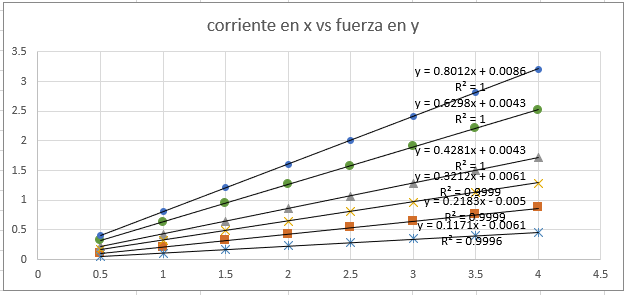
\includegraphics[scale=0.6]{../imgs/o.png}
   \caption{Corriente vs Fuerza}
   \label{Fig:1}
\end{figure}

En la figura \ref{Fig:1}, se pueden apreciar los datos obtenidos al comparar la corriente establecida en el circuito, con la fuerza que la misma generaba sobre una serie de imanes. En el gráfico se puede apreciar que todas las líneas generadas por los datos recabados resultaron en trazos lineales ascendentes, es decir, que fueron creciendo proporcionalmente a como iba aumentando la corriente inducida al circuito en cuestión.
\begin{figure}[H]
   \centering
   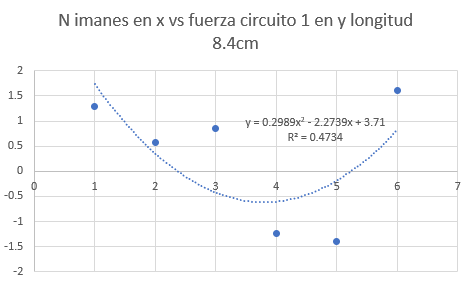
\includegraphics[scale=0.6]{../imgs/o1.png}
   \caption{Imanes vs Fuerza (1)}
   \label{Fig:2}
\end{figure}

En la figura \ref{Fig:2}, se realizan los gráficos con los parámetros del numero de imanes presente en el pesaje en comparación con la fuerza ejercida por el circuito sobre dichos imanes. En esta primera gráfica se pueden apreciar que los puntos marcados están dispersos y con una distribución variable, esto debido que al momento en que se realizó la medición, no se tomaron en cuenta la posición de los polos y afecto el valor medido, a pesar de que la corriente se mantuvo constante.

\begin{figure}[H]
   \centering
   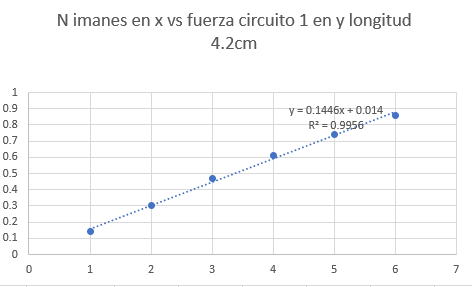
\includegraphics[scale=0.6]{../imgs/o2.png}
   \caption{Imanes vs Fuerza (2)}
   \label{Fig:3}
\end{figure}

En la figura \ref{Fig:3}, el gráfico fue realizado con los mismos parámetros que el anterior, solo que en este caso el trazo salió lineal y acorde a lo establecido en la teoría, esto debido a que en esta ocasión si se tomó en cuenta la posición en la que se encontraban colocados los polos de los imanes, haciendo que la medición resultará muchísimo más exacta y confiable que la anterior. De igual forma, el amperaje se mantuvo constante.

\begin{figure}[H]
   \centering
   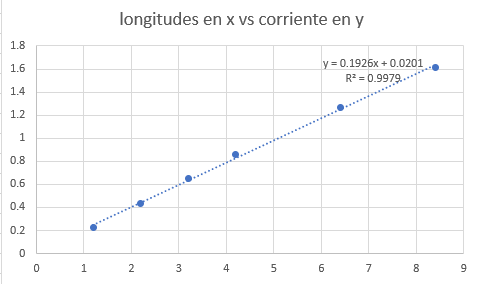
\includegraphics[scale=0.6]{../imgs/o3.png}
   \caption{Longitud vs Fuerza}
   \label{Fig:4}
\end{figure}

En la figura \ref{Fig:4}, los parámetros establecidos en el gráfico fue la longitud del circuito y la fuerza ejercida por el mismo a la balanza. En este caso, los circuitos fueron variando según la longitud que tuvieran, mientras que la corriente inducida al mismo circuito se mantuvo constante, resultando en un trazo lineal,  haciendo ver que el tamaño del circuito afecta directamente en la fuerza producida por la corriente, aún cuando esta se mantenga constante.



\section{Conclusiones}\label{Conclusiones}				% -------------------- Conclusiones
El objetivo si se cumplió, la teoría se asemejo muy bien a la práctica y como se pudo observar en las gráficas y como ya mencionado el comportamiento de nuestros datos es el correcto a excepción de cuando volteamos los polos, por otro lado y como ultimo comentario
se ha desarrollado teóricamente la expresión de la fuerza de Lorentz dependiendo del sistema de referencia, distinguiendo entre la forma en reposo y en movimiento de la partícula cargada. Esta cuenta con una importancia fundamental en electromagnetismo y mecánica cuántica.

\begin{thebibliography}{9}						% -------------------- Bibliografía
	\bibitem{Fernandez}
 Fernández, J. L. (s. f.). Ley de Lorentz. Fisicalab. https://www.fisicalab.com/apartado/ley-de-lorentz
	\bibitem{Serway}
	Serway, R. A., $\&$ Jewett, J. W. (2008). Física para ciencias e ingeniería. (7.a
ed., Vol. 1). CENGAGE Learning.

\bibitem{Pérez}
	Newton, I. (1687). Philosophiæ Naturalis Principia Mathematica [Mathematical Principles of Natural Philosophy]. Londini: Jussu Societatis Regiæ ac Typis Josephi Streater.

\end{thebibliography}
\end{document}	